% !TEX root = ../stellar-notes.tex

\DefineShortVerb{\|}

\begin{mesaproject}[Convection in a pre-main-sequence star]
\label{m.MESA-convection}

For this exercise, we'll use the setup from MESA Experiment \ref{m.MESA-contraction}, namely a contracting, pre-main-sequence star of mass $\val{1}{\Msun}$.  Download the folder |convection/1M-convection| and place it into your projects folder. 

For this exercise, we don't need any custom output, so we are just using the standard '|run_star_extras.f90|' file.  We still need to compile the code, however, so do `|./mk|'. We will also need a starting model. We created a model of a fully convective pre-main-sequence star with $M = \val{1}{\Msun}$ in Experiment \ref{m.MESA-contraction}. Copy the saved file `|1M_PMS.mod|' into your work folder `|1M-convection|'.

The first thing we want to plot is the entropy in the star. If we look at the file `|$MESA_DIR/star/defaults/pgstar.defaults|', we notice that |Profile_Panels1| is close to what we want: its first panel plots both $\log(T/\K)$ and  $S/(\NA\kB)$. We don't need the second panel, though, so we'll make the following changes to `|inlist_pgstar|'.  We'll swap out the `|TRho|' plot for `|Profile_Panels1|', and then we'll set the number of panels to be just 1.  The following lines of |inlist_pgstar| accomplish this:
\VerbatimInput[firstline=36,lastline=39]{convection/1M-convection/inlist_pgstar}
The defaults for the rest of the settings for `|Profile_Panels1|' are fine, so we don't need to set them explicitly.
Now when you do `|./rn|' the window will have a plot of both entropy and temperature as functions of enclosed mass in the lower left panel.

\begin{exercisebox}[Entropy profile of star]
\begin{enumerate}
\item Compare the entropy profile when the star is fully convective, and when a radiative region develops as it approaches the main sequence. Does the profile match your expectation given in the warm-up exercise?
\item Look at $\log[T(m)]$. In Ch.~1 of the notes, we discuss estimates of the interior temperature, and we often use the central value as a representative value.  Is this reasonable? Make this quantitative: at the point when the star joins the main sequence, find the mass at which $\log[T(m)] = \log[T_{c}]-0.5$ and $\log[T(m)] = \log[T_{c}]-1.0$.
\end{enumerate}
\end{exercisebox}

\subsection{Convective efficiency}

We argued in \S~\ref{s.efficiency-convection} that convection was very efficient in the solar interior.  By efficient, we mean that a very slow convective velocity $v_{\mathrm{conv}}$ is sufficient to carry the flux.  As a result, the difference between the temperature gradient and the adiabatic one is also expected to be very small: $\nabla - \nablaad \ll 1$, where $\nabla \equiv \dif\ln T/\dif\ln P$ and $\nablaad=(\partial\ln T/\partial\ln P)_{s}$. We also worked through a linear stability analysis in \S~\ref{s.convection-second-look} and found (eq.~\ref{e.blob-eq-of-motion}) the \emph{Brunt-V\"ais\"al\"a} frequency $N^{2}$. This is the oscillation frequency for a fluid element that is adiabatically displaced in the radial direction; $N^{2}< 0$ in a region with $\nabla > \nablaad$ and therefore unstable to convection.

For this project, you are going to examine $\nablaad$, $\nablaad-\nabla$, $N^{2}$, and $v_{\mathrm{conv}}/c_{s}$. In the first assignment, we had to customize `|run_star_extras.f90|' to output specific quantities, but in this case the information we want is already computed by \mesa. A complete listing of the quantities available for each zone is in `|$MESA_DIR/star/defaults/profile_columns.list|'. Browsing this list, we see that `|grada|' ($\equiv \nablaad$) and `|conv_vel_div_csound|' ($\equiv v_{\mathrm{conv}}/c_{s}$) are both written by default to `|profile|\emph{dd}|.data|'; the other two variables are computed by \mesa, but are not, by default, written to file (in `|profile_columns.list|' they are commented out, i.e., preceded by a bang `|!|').  To enable the printing of these two variables, we set, in the `|star_job|' section of the `|inlist_1M_convection|', the flag
\VerbatimInput[firstline=20,lastline=20]{convection/1M-convection/inlist_1M_convection}
which loads a list of profile variables from the file `|convection_variables|'. This file first loads the defaults
\VerbatimInput[firstline=18,lastline=19]{convection/1M-convection/convection_variables.list}
and then loads a useful coordinate (used later) `|logxq|', defined as $\log(1-q)$ with 
$q = m(r)/M$.
\VerbatimInput[firstline=22,lastline=22]{convection/1M-convection/convection_variables.list}
The file finally loads the remaining four variables $\nablaad$, $\nablaad-\nabla$, $N^{2}$ (scaled), and $v_{\mathrm{conv}}/c_{s}$:
\VerbatimInput[firstline=24,lastline=33]{convection/1M-convection/convection_variables.list}

With these four quantities now being written to the profile data, we can plot them.  I've copied a template for this, which uses the `|Profile_Panels6|' variables, into the file `|inlist_convection_vars|'. You will need to customize this to produce the desired plot.  There are many ways to plot the four variables. Figure~\ref{f.convection} shows one; see if you can duplicate it! Note that in making this plot you might have to set the minima and maxima for the plots; for some of these quantities the values near the surface are at a very different scale than throughout the bulk of the star.  We will look in more detail at what happens near the photosphere in the next exercise.

\begin{figure}[htbp]
\centering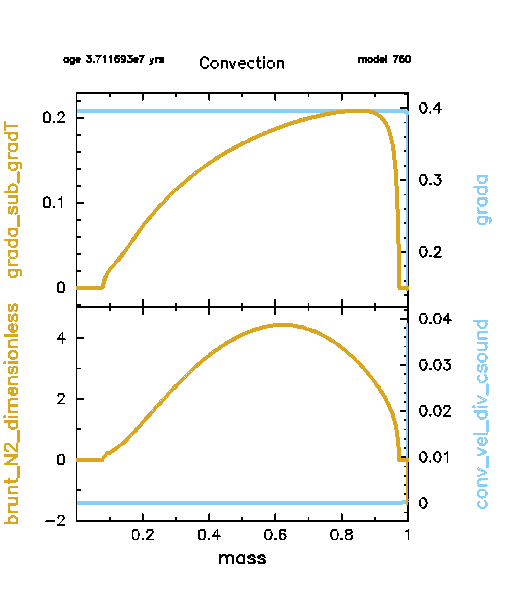
\includegraphics[width=0.8\textwidth]{Convection_000760}
\caption{\label{f.convection}
Snapshot of convective variables throughout the star.}
\end{figure}

\newthought{Tip:---Unlike the parameters} in `|&controls|' and `|&star_job|', the settings in 
`|&pgstar|' are reread at each step.  This means you can change parameters, such as the minimum and maximum values for axes, while the program is running!  To pause the program execution during an interactive run, type `|ctrl-z|'; you should then get a message such as
\begin{Verbatim}
^Z
[1]+  Stopped                 ./rn
\end{Verbatim}
To restart, type `|%1|'
(where the `|1|' is whatever number precedes the word `|Stopped|').

\begin{exercisebox}[The adiabatic temperature gradient]
\begin{enumerate}
\item How does the value of $\nabla_{\mathrm{ab}}\equiv (\partial\ln T/\partial\ln P)_{s}$ compare with the value expected for an ideal gas?
\item The Brunt frequency $N^{2}$ that is plotted is actually in units of $3GM/R^{3}$; explain from the derivation in the notes why the factor $GM/R^{3}$ is sensible.  What is a characteristic value of $N$ (when the star has approached the main sequence and most of the star is not convective)?
\end{enumerate}
\end{exercisebox}

\subsection{Approaching the photosphere}

As you will notice from these plots, there is a lot happening for $m(r) > \val{0.99}{\Msun}$, but all of the action is compressed against the right-hand side of the plot.  Wouldn't it be nice to rescale the x-axis to zoom in on this region?  Fortunately, there is an easy way to do this.  \mesa\ defines a variable $q = m(r)/M$, and one of the variables written out by default is `|logxq|', defined as $\log(1-q)$. Since $q$ ranges from $0$ at the stellar center to $1$ at the surface, `|logxq|' is $0$ at the center and goes to a very large, negative number near the surface. This means that the surface will be at the left-hand edge of the plot and the center at the right, so the orientation is opposite to plots using `|mass|' or `|radius|' on the x-axis.  You can switch the orientation of the x-axis by setting `|Profile_Panels6_xaxis_reversed = .true.|'.

\begin{exercisebox}[The adiabatic gradient near the surface]
\begin{enumerate}
\item Re-run the evolution, this time setting the x-axis to `|logxq|' for the plots of $N^{2}$, $v_{\mathrm{conv}}/c_{s}$, $\nablaad$, and $\nablaad-\nabla$.  Setting
\begin{Verbatim}
   Profile_Panels6_xmin = -12
   Profile_Panels6_xaxis_reversed = .true.
\end{Verbatim}
is a good choice here. You will notice that $\nablaad$ behaves in an interesting fashion in the outer regions of the star.  Do $\rho$ and $T$ take on any characteristic values at the location of the feature?  Hypothesize about what may be happening there.
\end{enumerate}
\end{exercisebox}

\subsection{What to turn in}
Make plots for models when the center of the star first becomes radiatively stable, and when the star reaches the main sequence.  To have the plots written to a file, set
`|Grid1_file_flag = .true.|' and '|Profile_Panels6_file_flag = .true.|'.  Make sure that the flags `|Grid1_file_dir|' and `|Profile_Panels6_file_dir|' are both set to `|frames|'.  There is no need to generate a plot for each timestep; you can set the interval between plots via `|Grid1_file_interval|' and `|Profile_Panels6_file_interval|' (I set them to be 10).

\end{mesaproject}

\UndefineShortVerb{\|}
